\documentclass[12pt,a4paper,onecolumn]{article}

% Encoding and language
\usepackage[utf8]{inputenc}
\usepackage[T1]{fontenc}
\usepackage[english]{babel}

% Font
\usepackage[sfdefault]{carlito}
\usepackage[normalem]{ulem}

% Set margins
\usepackage[a4paper, top=2cm, bottom=2cm, left=2.5cm, right=2.5cm]{geometry}

% Tabulation
\usepackage{tabto}

% Line spacing
\usepackage{setspace}
\onehalfspacing

% Page numbers
\usepackage{fancyhdr}
\pagestyle{fancy}
\fancyhf{} % Clear default header/footer
\rfoot{\thepage} % Right-aligned page numbers in footer

% Remove page number from cover/abstract/etc
\usepackage{titlesec}
\newcommand{\noPageNumber}{\thispagestyle{empty}}

% Prevent indentation
\setlength{\parindent}{0pt}
\setlength{\parskip}{0.5em}

% Table
\usepackage{booktabs}

% Figure management
\usepackage{graphicx}
\usepackage{caption}
\usepackage{subcaption}
\usepackage{wrapfig}

\usepackage{pgfplots}
\pgfplotsset{compat=1.16}
\def\mathdefault#1{#1}
\everymath=\expandafter{\the\everymath\displaystyle}

% Subfigure management
\usepackage{layouts}
%\usepackage{floatrow}
%\usepackage[label font=bf,labelformat=simple]{subfig}% <-- changed
%\floatsetup[figure]{style=plain,subcapbesideposition=top}


% Optional: headings formatting
\titleformat{\section}{\large\bfseries}{\thesection}{1em}{}
\titleformat{\subsection}{\normalsize\bfseries}{\thesubsection}{1em}{}

% Optional: remove widow/orphan lines
\widowpenalty=10000
\clubpenalty=10000

% Mathematics
\usepackage{amsmath,mathtools,amssymb} 

% References
\usepackage[backend=biber, style=authoryear]{biblatex}
\addbibresource{Bibliography.bib}

\usepackage{hyperref}
 

\begin{document}
 %% textwidth in cm: \printinunitsof{in}\prntlen{\textwidth}

\begin{titlepage}
   \begin{center}
      
\includegraphics[width=0.65\textwidth]{logos.png}
      

       \textbf{\Huge Gap year Internship Report}

       \vspace{0.5cm}
       \LARGE Evaluating the impact of maturation time variability in stage-structured host-parasitoid models.
            
       \vspace{1cm}

       \textbf{Mathis Drieu}

        \vspace{1cm}
        \normalsize
        Under the supervision of\\
        Quentin Guilloit, Jules Guilberteau, Thierry Spataro
        \vspace{0.5cm}

        
        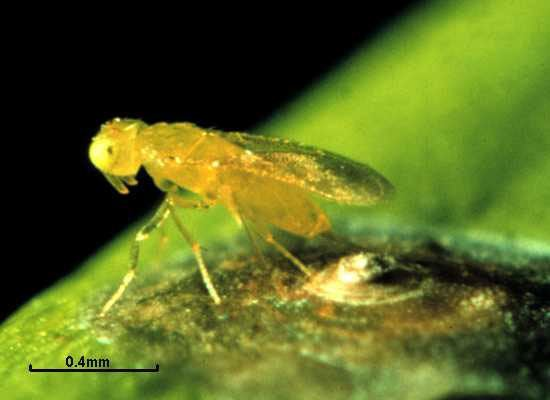
\includegraphics[width=0.70\textwidth]{aphytis-melinus.jpeg}
        \small\textnormal\\
        Parasitoid \textit{Aphytis melinus} and its host \textit{Aonidiella aurantii}, a pest of citrus in California and elsewhere (Alchetron encyclopedia).
       
       
       \vspace{0.5cm}
        \large   
       IEES, Sorbonne Université\\
       Team DYNECO\\
       \normalsize February-June 2025\\
       
            
   \end{center}
\end{titlepage}

\newpage

% Abstract (no page number)
\noPageNumber
\begin{abstract}

Biocontrol, i.e. the use of insect parasitoids, is a nature-based agronomical lever that can help limiting crops pest populations and reduce agricultural dependency to insecticides. Insect host-parasitoid models are crucial tools to better understand and manage pest populations, especially in the context of biocontrol. Such models often assume either fixed (no developmental variability) or exponentially distributed maturation times (high developmental variability). Here, we investigate intermediate cases using Erlang-distributed delays via the linear chain trick, applied to classical host-parasitoid systems with diverse dynamics. We find that while developmental variability generally stabilizes population dynamics, model sensitivity varies, and abrupt changes in behavior can occur at both low and high variability levels. We conduct a review of empirical data from laboratory-reared agricultural insects, fitting Erlang parameters to quantify developmental variability. This analysis reveals substantial heterogeneity across species and suggests that exponential assumptions might often be unrealistic. We also examine the effect of maturation-time shifts, accounting for periods during which no maturation can occur, showing that omitting such shifts during fitting systematically lowers estimated variability. Taken together, our results support interpreting developmental variability as a form of parasitism risk heterogeneity, with stabilizing effects comparable to those of spatial heterogeneity, such as patchiness. We argue that developmental variability deserves comparable attention, particularly given its tractable mathematical implementation via the linear chain trick and, more broadly, through phase-type distributions.

\end{abstract}

% Table of Contents, List of Abbreviations (no page numbers)
\noPageNumber
\tableofcontents


% Main content starts here (with page numbers from 1)
\newpage
\setcounter{page}{1}






\section{Introduction}

\tabto{1 cm} Individuals interact with their environment sometimes as a function of their age, size or physiological state that varies during their life. For example, the ability to consume or predate some resources, intra-specific competition, as well as predation/parasitism risk can differ across size classes or life stages. This is particularly salient for insect species, and notably the holometabolous clade which has a discontinuous development made up of eggs, larvae, pupae, and the imago (or adult). Stage-specific processes, such as larval-specific parasitism by parasitoids, can have deep consequences for the dynamics of the whole populations (Gurney 1998, cited by Robertson 2018). This has sustained the need to account for age or size structure in population models, typically through phenological  structured models of insect populations,which are crucial study systems in insect pest management (Birt 2009, Fauvergue 2020). \\

dH/dt = R(t) - M(t) \\
\tabto{1 cm}  A variety of approaches exist to model populations with strutured life-cycles and comes with a trade-off between simplicity and realism.\\

\tabto{1 cm} Cf Séparer les stades biologiques réels et les lumping méthodologiques.  \\


\tabto{1 cm} Generally, stage-structured models of populations lump together groups of age or size with common characteristics (Gurney 1983). In discrete time, Lefkovich (Lefkovich, 1965) and Usher (SOURCE?) matrix models have been used to study stage/size-structured populations’ dynamics with non?-overlapping generations. In continous time stage-structured models, two main frameworks have been used. On the one hand, modelers have frequently \textcite{robertson_matter_2018} relied on the per-capita rate of transition from one compartment to another. More precisely, in the case of stage-structured models, they have used the per-capita developmental rate. This results in Ordinary Differential Equation (ODE) type models. They are highly tractable and associate each transition to one parameter, the per-capita developmental rate, classically computed as the inverse of the average developmental time. On the other hand, in line with the work of \textcite{gurney_systematic_1983}, many modelers have directly used this average developmental time as a fixed lag governing the transition from one stage to another. This results in Delayed Differential Equations (DDE) type models. About half of the stage-structured models found in recent literature use the ODE models, while most of the second half use DDE models. \textcite{robertson_matter_2018}. This dominance can be explained by their simplicity: ODEs offer high tractability and low computational cost; and both approaches only require to know the average stage duration. Yet, they differ fundamentally in how they represent inter-individual variability in stage duration. \\

\tabto{1 cm}  Indeed, all the mentioned approaches does not allow to control the inter-individual variability of developmental time in the (stage) population, yet it was shown to deeply influence population dynamics. Variability will hereafter refer to the coefficient of variation (CV) of a metric, defined as its standard deviation divided by its mean in a population. Matrix and ODE models implicitly assumes that maturation time follows a geometrical (discrete time) or exponential (continuous time) distribution (Birt 2009, Hurtado 2019). At population scale, this implies that the average maturation time is equal to its variance (CV = 1). At individual scale, this unrealistically implies that the probability of transition is maximal at the entrance of the stage. Conversely, DDE models assume that all the individuals of a given cohort maturing synchronically. In other words they assume a null maturation time variance (CV = 0). This variance can have deep consequences for population dynamics (de Valpine 2014, Eurich 2005). Populations and communities are usually destabilized by fixed delays between stages (SOURCE : bcp de choses générales sur les délais en modélisation/les str en stage), and the addition of maturation time variability sometimes counteracts this effect (Eurich 2005, Beretta 2016). Indeed, this variability frequently increases stability and persistence of populations (Eurich 2005), and notably so  in host-parasitoid population dynamics (Smith and Mead 1974, Blythe et al 1984, Wearing 2004, Nakamichi 2008, Cronin 2016). Thus, ODE and DDE models [may?] sacrifice realism for simplicity by imposing developmental time distributions with fixed CVs of either 0 or 1. Such hidden assumptions may yield critically inaccurate predictions of population dynamics (Wearing 2004, Xu et al. 2010).  \\


\tabto{1 cm}  The Linear Chain Trick (LCT) is a modeling method which allows to relax these extremal assumptions. By dividing a stage into n sub-stages, this trick allows modeling Erlang-distributed developmental times, where their coefficient of variation CV are equal to $1/\sqrt{n}$. The LCT allows to relax the hypothesis on DTV of ODE and DDE approaches, which are then captured as two extremas. Indeed, the “ODE” approach is equivalent to a “LCT” approach with n = 1 substage (CV = 1), while the “DDE” approach is equivalent to a “LCT” approach with an infinite number of substages (CV = 0). Thus, this framework bridges the gap between ODEs (n=1, CV=1) and DDEs (n$\rightarrow \infty$, CV=0), enabling intermediate variability that may be both more plausible and tractable (Hurtado?), at the cost of only one additional parameter, the number of substages n. Although it consists in increasing the number of equations, the LCT yields ODE-type models, which are substantially easier to [algebraically] analyse and simulate than DDE systems and a fortiori IDE systems.Along with its discrete time equivalent for matrix models (Birt 2009), this Linear Chain trickery has been increasingly used in ecological (Smith and Mead 1974, Wearing 2004, Bjornstad et al. 2016, Nelson et al. 2019, Cavani 2022) and epidemiological studies (Wearing 2005, Hurtado 2019), but its adoption remains fragmented and poorly documented. Many applications use the LCT cryptically, with little explanation of its implementation (e.g., Murdoch 2005, Mermer et al. 2020, Rincon et al. 2023). Moreover, its utility remains unclear: When does accounting for DTV via LCT meaningfully improve model predictions? Put more bluntly, when should modelers pain themselves to use the LCT instead of either simple ODE (n=1) or DDE approaches? And how does empirical DTV in insects compare to the assumptions of ODE,DDE and LCT models? \\

\tabto{1 cm}  This uncertainty persists for two reasons. First, while the effects of DTV on dynamics are well-studied (e.g., stabilization in host-parasitoid systems), the cost-realism trade-off of implementing the LCT has never been systematically assessed. Second, the effect of DTV has not been systematically related to a unified summary of empirical developmental time variability, particularly for insect species related to pest management (but see : Xu et al. 2010). Here, we address these gaps by combining theoretical and empirical analyses with a focus on insect population models. We apply the LCT to two landmark and strategic (sensu Levins, 1966) models: 1. a single-species model with cohort competition (Gurney 1980) ; and 2. a host-parasitoid system (Murdoch et al. 1987). We thereby aim to quantify, using the LCT and a range of subcompartment number n values, how developmental variability affects population dynamics and equilibriums. We also survey empirical development time data from insect pest management literature, extracting CVs and mapping them to the corresponding n values for the LCT. This dual approach allows us to (1) assess the sensitivity of population dynamics to DTV, and (2) evaluate the realism and use simplicity of LCT relative to ODE/DDE frameworks. We show that the use of the LCT on ecological models may be easy and does not critically hamper algebraic analysis [en vrai valeurs propres à calculer : relou, et analyse algébrique devient vite impossible] and numerical simulation. We also show that [empirical developmental variability is diverse and not realistically captured by fixed delay, and a fortiori exponential distribution (CV=1) assumptions. On the contrary, Erlang distributions, provided with the right parameters, frequently match closely with empirical developmental time distributions. These results indicate that [LCT is practical and DTV is important : we encourage modelers to use it]. 


Hereafter, maturation time variability will be understood as the the coefficient of variation (CV) of the maturation time, i.e. its standard deviation divided by its mean. Dividing by the mean yields a dimensionless measure that reflects the variability of the maturation time, independently of its average.


\section{The LCT as a way to control developmental time variability in stage-structured models}


\section{App 1}

\subsection{Isolated insect population with negative cohort competition}

\subsection{Host-parasitoid interaction with juvenile host parasitism}
\tabto{1 cm} We consider the continuous-time host-parasitoid model detailed in Murdoch et al. 1987 in a DDE approach. The host and parasitoid life cycles are divided into 2 stages: juvenile ($H_1, P_1$) and reproductive adult ($H_2, P_2$). Parasitism could occur on either of the host two stages, but we use the model where the juvenile, non-reproducing, stage $H_1$ is vulnerable to parasitism. Parasitoids search randomly and independently at rate $a$ such that the per-capita rate of $H_1$ mortality from parasitism is $aP_2(t)$. Adults die through a constant mortality rate, which means that the adult lifespan follows an exponential distribution. There is no density-dependent component in host mortality. It can be justified by the fact that host populations are much below the level where food or other resources can be limiting if the pest (bio)control is successful (Murdoch 1987). Except for the parameters used in Figure 2c, the temporal scale is normalized by the maturation time of the host: $m_H = 1/T_{H1}$ are set to 1. The application of the LCT to obtain a distributed-delay model as close as possible as the fixed-delay model introduced by Murdoch is detailed in Appendix A.1. These constructed models, which vary according to the used number of subcompartments \textit{n} and \textit{m}, will be named "LCT-ODE" models.


\begin{wrapfigure}{l}{0.5\textwidth}
\centering
\includegraphics[width=0.5\textwidth]{../../model_host_parasitoid/figs/Murdoch_box_system2.pdf}
\caption{The LCT-ODE host-parasitoid model based on the model described in Murdoch (1987). H1 and P1 population densities are equal to $\sum_{i=1}^{n} H_{1,i}(t)$ and $\sum_{i=1}^{m} P_{1,i}(t)$.}
\label{fig:system}
\end{wrapfigure}

\tabto{1 cm} A spectrum of LCT-ODE models is obtained, including the case where the number of subcompartments is 1, i.e. the exponentially-distributed model (Figure 1). The resulting LCT-ODE system of equation is given by equation (1) (or (8) in Appendix), with notation $\dot{X} := \frac{dX}{dt}$. \\

\tabto{1 cm} In all models, the mean development times are set equal. Although the proportion of juvenile survival can be equalized (future publication of J.Guilberteau), the parametrization was kept simple. Ignoring juvenile intrinsic mortality,  the constraint on the mean development time gives (in the case of the host, the parasitoid has an analogous formula) $\theta_H = n \times m_H = n/T_{H1}$. With this parametrization, the proportion of juvenile survival depends on \textit{n} (see Appendix and Discussion). Apart from this, the construction of the LCT-ODE model is made such that the only difference between all the models are maturation time variability. 

\begin{equation}
\begin{dcases}
\dot{H_{1,1}}(t) = H_{1,1}(t)(-a P_2(t) - \delta_{H1} - \theta_H) + r H_2(t) \\
\vdots \\
\dot{H_{1,i}}(t) = \theta_H(H_{1,i-1}(t) - H_{1,i}(t)) - \delta_{H1} H_{1,i}(t) - aP_2H_{1,i}(t), \quad i \in (2, 3, \dots, n) \\
\vdots \\
\dot{H_{2}}(t) = \theta_H H_{1,n}(t) - \delta_{H2} H_{2}(t) \\
\dot{P_{1,1}}(t) = P_{1,1}(t)(- \delta_{P1} - \theta_P) + a P_2(t) \sum_{i=1}^{n} H_{1,i}(t) \\
\vdots \\
\dot{P_{1,i}}(t) = \theta_P(P_{1,i-1}(t) - P_{1,i}(t)) - \delta_{P1} P_{1,i}(t), \quad i \in (2, 3, \dots, m) \\
\vdots \\
\dot{P_{2}}(t) = \theta_P P_{1,m}(t) - \delta_{P2} P_{2}(t) \\
\end{dcases}
\end{equation}

\tabto{1 cm} The local stability of the non-trivial equilibria of the system is  analyzed using linear stability theory. Specifically, the characteristic equation derived from the linearized system at each equilibrium point yields a set of roots. These roots correspond to the eigenvalues of the jacobian matrix in the case of a ODE-type system. The real parts of these roots determine the local behavior of the system near the equilibrium. If all the eigenvalues of the Jacobian matrix evaluated at any equilibrium point have strictly negative real parts, then the corresponding equilibrium is locally asymptotically stable. Conversely, if at least one eigenvalue has a positive real part, the equilibrium is unstable. 
\tabto{1 cm} Local stability diagrams are be generated. They map out regions of parameter space where specific equilibria are stable or unstable. These diagrams are built by systematically computing the Jacobian matrix across a grid of parameter values and analyzing the sign of the real parts of its eigenvalues. When an eigenvalue's real part crosses 0, a boundary is drawn. Here, the two parameter axes will be the longevity of the adult host $T_{H2} := 1/\delta_{H2}$ and the maturation time of the parasitoid $T_{P1} := 1/m_P$ which were found to have a strong impact on stability. The diagrams were generated using the function Eigenvalues of Wolfram Mathematica (Version 14.1) applied to the Jacobian matrix of the LCT-ODE system. 
\tabto{1 cm} Bifurcation diagram are also generated. These diagrams show equilibria or periodic solutions as functions of a  parameter, highlighting points where stability changes (i.e. bifurcations). By giving information about the periodic solutions when the asymptotic behavior of the model are limit cycles, bifurcation diagram are complementary to local stability diagram. To characterize these oscillations, numerical simulations were realized using the Mathematica function NDSolve with an automatic (and dynamically changing) solver method. In the light of the frequent stiffness issues of the simulations, NDSolve was found to offer the most fast and reliable solver compared to other tested methods with various Python libraries. For further details, relevant Mathematica and Python scripts can be found on Github.\\

\begin{figure}[!ht]
\centering
\includegraphics[width=\textwidth]{../../model_host_parasitoid/figs/Murdoch_equilibrium.pdf}
\caption{Effect of maturation variability on the values of the non trivial equilibrium densities in two host-parasitoid models. \textbf{(a)} : Non trivial equilibrium densities (noted $X^*$ for each stage X) of Murdoch system as a function of the Erlang distribution shapes \textit{n} and \textit{m}. See Figure 3 for parameters values.}
\label{fig:Eq_densities}
\end{figure}


\begin{figure}[!ht]
\centering
\includegraphics[width=\textwidth]{../../model_host_parasitoid/figs/Murdoch_stability_diagram.pdf}
\caption{Effect of maturation variability on the stability properties of the Murdoch 1987 model. Remind that $n = 1/CV_{\text{maturation time of H1}}^2$. Parameters are $\delta_{H1} = 0, \delta_{P1} = 1, \delta_{P2} = 8, \rho = 33, a = 1, m_P = 1$. \textbf{(a)} : Local stability diagram of the system around the non-trivial equilibrium. The system is unstable to the left of the curves, and stable to their right.}
\label{fig:Murdoch}
\end{figure}



\tabto{1 cm} Using fixed delays, Murdoch et al. (1987) showed that the invulnerability of the host adult reproductive stage stabilizes the system because this stage constitutes a "refuge" to parasitism mortality. In line the longevity of the adult host was found to be the main stability factor of the system. In the present work, maturation variability was added through the construction of a LCT-ODE (with \textit{n} subcompartments for $H_1$ and  \textit{m} subcompartments for $P_1$) system with average developmental times equal to those of the Murdoch's DDE system.
\tabto{1 cm} Let us evaluate the effects of developmental variability on the stability of the non-trivial equilibrium. In the ODE framework (\textit{n} = \textit{m} = 1), it is almost always stable, except for a short range of low $T_{H2}$ values (Figure 3a). The unstable area increases as \textit{n} and \textit{m} increase and does not change much after they attain values around 20 or 30 (Figure 3a). The bifurcation diagram (Figure 3b) specifies the oscillation properties of the system. In addition to causing the reduction of the area of unstability, developmental variability causes the increase of the amplitude and the period of oscillations. The extent of this effect is dependent of the chosen parameters (Supplementary Figure 1).



\tabto{1 cm} Developmental variability (smaller values of \textit{n} and \textit{m}) causes the non-trivial equilibrium densities to increase, except for the case of $H_1$ (Figure 4a). The increase is particularly sharpe for small values of \textit{n}. For instance, between \textit{n} = \textit{m} = 5 and \textit{n} = \textit{m} = 1, The adult host equilibrium density $H_2^*$ is multiplied by 5 for this set of parameters. Between \textit{n} = \textit{m} = 100 and \textit{n} = \textit{m} = 10, the ratio reduces down to 1.13. 

\tabto{1 cm} Host fecundity is stabilizing at very high maturation variability (\textit{n}=1 or 2, Figure 5a) and destabilizing otherwise (Figure 5b). Developmental variability of both the host and the parasitoid increase the area of stability in a similar and additive way (Supplementary Figure 2). Parasitoid's developmental variability does not reverse the effect of fecundity on stability (Supplementary Figure 3). Together, these results indicate that maturation variability is indeed a stabilizing factor and can modulate the effect of other demographic parameters (here fecundity) on stability. 


\section{App 2}

\tabto{1 cm} Wagner et al. (1984) introduced a method to fit a Weibull distribution to normalized maturation time of individually marked insects bred in laboratory at various temperatures. Their method contributed to establishing the Weibull distribution as a standard tool for estimating variability in insect maturation times. The Weibull and Erlang distributions can be visualized in Figure 2. They are equal for a shape equal to 1. They both converge to a dirac distribution when their shape goes to infinity. 

\begin{figure}[!ht]
\centering
	\begin{subfigure}[t]{0.48\textwidth}
	  \centering
	  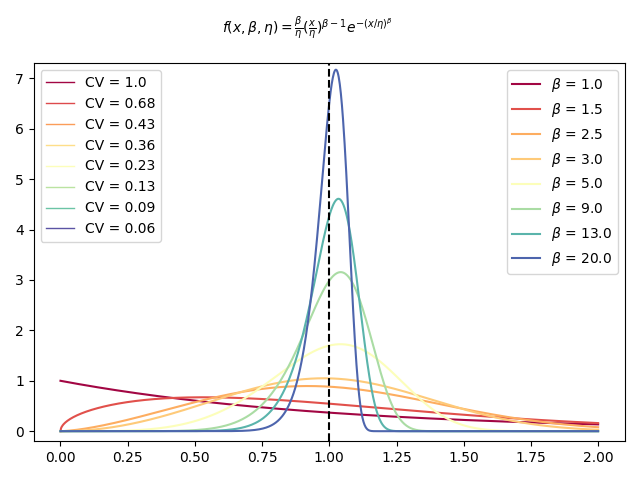
\includegraphics[width=\textwidth]{../../survey_gamma_shape/figs/weibull_distribution.pdf}
	\end{subfigure}
	\hfill
	\begin{subfigure}[t]{0.48\textwidth}
	  \centering
	  \includegraphics[width=\textwidth]{../../survey_gamma_shape/figs/gamma_distribution.pdf}
	\end{subfigure}

\caption{Weibull (left) and Erlang (right) distributions for various shapes as well as their respective probability density function. The respective Weibull and Erlang shapes are $\beta$ and n. The respective Weibull and Erlang rates are $\eta$ and $\theta$, and were set to fix the esperance of the distribution to 1. Line colors are set according to the value of the coefficient of variation CV (standard deviation / mean) of the given distribution.}
\label{fig:distributions}
\end{figure}

\tabto{1 cm} In their method, times are normalized (divided) by the median maturation time at the given temperature, the distribution is built to only represent the variability of maturation time (independently of its mean). Xu et al. (2010) reviewed the literature using Wagner's method. The raw data of insects' developmental times are rarely provided in the papers. The Weibull estimates are thus a practical and condensed set of information about empirical maturation variability. Xu et al. (2010) thus gathered the Weibull parameters of various insects' developmental stages, and simulated 5000 time variates from the given Weibull laws. Then, they fitted a Gamma law by finding the Gamma parameters that maximize the likelihood of the simulated data. 
\tabto{1 cm}  Here, the same method was applied. Like Xu et al., the literature review was conducted on the papers that cite the original Wagner's (1984) paper. Our review is not exhaustive but adds several (around 20) relatively recent papers to Xu et al.'s survey (also made up of around 20 papers). Similarly to Xu et al., the majority of the estimates were obtained on pest species of some economic importance as well as on their natural enemies. The dataset involves one parasitoid (\textit{Cotesia Melanoscela}, Gould and Elkinton 1990). Despite our use of Erlang laws in the modeling part, we will let the fitted Erlang shape to be non-integer in this part of our study. Therefore, in this part, we will be referring to a Gamma (and not Erlang) distribution. We will still use the notation \textit{n} to designate the Gamma distribution shape. Both distribution can be endowed with a third parameter, a shift $\tau$. This positive parameters shifts the distribution to the right, thereby producing a window of time where no maturation can occur. Most reviewed papers report a non-null shift. Since maturation times are normalized by their median, $\tau$ represents a proportion of the total development time and is allowed in $[0;1]$. The Gamma shape fit was conducted according to three constraints on the shift of the fitted Gamma law : it was estimated either in the range [0;1],  forced to 0, or assumed equal to the Weibull shift ("copied", like in Xu et al. (2010)). Contrary to Xu et al. (2010), combined stages were not eliminated. Tables and Python (Python 3.12.2) script summarizing the survey can be found on Github. 
\tabto{1 cm} The goodness-of-fit of the Gamma parameters estimation from Weibull parameters was evaluated in two ways. First, visualization plots superimposing the simulated Weibull time variates and the fitted gamma law were generated for each fit. They can all be found on Github. Second the Wasserstein-1 distance was computed for each couple of Weibull law and its corresponding fitted Gamma law. If each distribution is represented by a pile of soil, this metric can be thought as the amount of soil that needs to be moved times the mean distance it has to be moved. Wasserstein distance between a given distribution and the same one shifted by T is T. This metric is thus robust to similar-but-shifted distributions.




\tabto{1 cm} The developmental variability of laboratory-bred insects of agronomic interest was surveyed. A Gamma distribution was fitted to the reported Weibull law in the surveyed papers following the work of Wagner et al. (1984). A maximum likelihood method was used to find the 3 Gamma parameters: the shape $n$, the rate and the shift $\tau$. For the shift, the fit was conducted with 3 types of constraint : either the Gamma shift parameter ($\tau$) was forced to 0 ("$\tau = 0$"), either it was allowed in the range [0;1] ("$\tau \in [0;1]$"), or it was set equal to the given Weibull shift parameter ("$\tau$ copied"). 

\tabto{1 cm} The goodness-of-fit between the Weibull and Gamma distributions was estimated in two ways: with visualization figures superimposing the two laws, and with the Wasserstein distance between the two laws. The constraints "$\tau = 0$" and "$\tau \in [0;1]$" yield similar Wasserstein distances between the fitted Gamma distribution and the corresponding Weibull distribution (Table 1, Figure 8a). This group of constraint yields a mean Wasserstein distance superior by about 33\% to the mean distance associated with the third constraint ("$\tau$ copied") (Table 1). Conversely, the median Wasserstein distance associated with the first two constraints is inferior by about 30\% compared to the median distance associated with the third group. The inconsistent ordering between mean and median is caused by 5 sets of Weibull parameters that yield unusually high distances for the constraints "$\tau = 0$" and "$\tau \in [0;1]$", skewing their mean upward. These sets of parameters have a negative Weibull shift. With the constraint of a positive or null Gamma shift, the Maximum Likelihood method entails a very poor fitting of these distributions. The fits markedly improve when the Gamma shifts is allowed to be negative with the constraint "$\tau$ copied". For these reasons, these sets were ignored in the following analysis. Overall, the Wasserstein distances suggest that the goodness-of-fit is less variable when the shift is taken from the Weibull distribution, and that it is similar between the constraints "$\tau = 0$" and "$\tau \in [0;1]$" (Figure 8a). 


\begin{table}[h]
\centering
\begin{tabular}{lccc}
\toprule
\textbf{} & $\boldsymbol{\tau = 0}$ & $\boldsymbol{\tau \in [0,1]}$ & $\boldsymbol{\tau}$ \textbf{copied} \\
\midrule
Mean Wasserstein distance & 0.030 & 0.029 & 0.020 \\ 
Median Wasserstein distance & 0.013 & 0.012 & 0.016 \\\cmidrule{1-4}
Mean shift & 0.000 & 0.194 & 0.436 \\ 
Mean shape & 123.3 & 96.0 & 45.5 \\
Median shape & 57.9 & 31.3 & 6.2 \\
Max shape & 782.2 & 782.2 & 756.8 \\
Min shape & 4.5 & 1.9 & 1.8 \\
Low shape count ($\leq 20$) & 11 (19\%) & 24 (42\%) & 38 (67\%) \\
Significant shape change ($\tau=0$ vs $\tau \in  [0;1]$) & \multicolumn{2}{c}{20 (35\%)} & -- \\
\bottomrule
\end{tabular}
\caption{Summary statistics of the Weibull-to-Gamma distribution fitting across the three $\tau$ constraints.  62 sets of Weibull parameters were analyzed in total.  The 5 sets of parameters with negative shifts are included in the lines about Wasserstein distances, and excluded otherwise. A significant shape change is counted when the fitted shape differs by at least 1 between the 2 given constraints.}
\end{table}

\tabto{1 cm} The average Gamma shape is 22\% lower under the "$\tau = 0$" constraint than under the "$\tau \in [0;1]$" constraint (Table 1, Figure 8b). Similarly, the median shape is 46\% lower, the minimum shape goes from 4.5 to 1.9, and the proportion of low ($\leq 20$) shapes goes from 19\% to 42\%. The maximum shape is 782.2 with both constraints. The "$\tau$ copied" constraint is associated with markedly lower fitted Gamma shapes (Table 1, Figure 8b). 

\tabto{1 cm} The constraint of considering a null shift is associated with a higher fitted \textit{n}, as shown by the lines connecting the sets of points of the constraints $\tau = 0$ and $\tau \in [0;1]$ in Figure 8b. In line, A large original Weibull shift is associated with a large Gamma shape for the $\tau = 0$ constraint fits (Figure 8c). When the original Weibull shift is $\geq 0.8$, the fitted Gamma shape cannot be lower than around 50 (Figure 8c).. This suggests that the absence of maturation during the early phase of the stage is either taken into account through the shift ("$\tau \in [0;1]$" and "$\tau$ copied" constraints), or it is taken into account through a larger shape ("$\tau = 0$" constraint"). For 20 out of 57 fitted stages (35\% of cases), the difference between the fitted n with constraint $\tau = 0$ and the fitted n with constraint $\tau \in [0;1]$ is superior to 1. In all three fitting constraints, an originally higher Weibull shift is significantly associated with a lower Wasserstein distance between the fitted Gamma distribution and its corresponding Weibull distribution (Linear regression estimated with Ordinary Least Squares method, Wald test with all 3 p-values < 0.001) (Figure 7d). This suggests that even with the constraint to have a null Gamma shift, a large Weibull shift does not entail a poorer fit according to the chosen distance metric.














\section{Discussion}

XX





% References (excluded from page count) \textcite{w_w_murdoch_invulnerable_1987}
\printbibliography[heading=bibintoc, keyword={main}, title={References}]

% Appendix (excluded from page count)
\newpage
\noPageNumber
\appendix
\section{Appendix}
\setcounter{equation}{0}

\subsection{Murdoch 1987 system}
\subsubsection{System construction : application of the Linear Chain Trick with a non-autonomous mortality term}
Note that Hurtado et al. 2018 as well as Lou and Sun 2022 give detailed justifications about the construction of continuous stage-structured models with an arbitrary maturation distribution and their convergence to a coupled system of ODEs in the case of the Erlang distribution. However, they do not include a non-autonomous mortality term. Let us thereby justify thoroughly how the studied LCT model was built analogously to the DDE model given by Murdoch (1987).

Let us consider the general form of the models used both in the ODE and DDE framework:
\begin{equation}
\dot{H_{1}}(t) = B(t) - M_n(t) - \delta(t, ...) H_1(t).
\end{equation}

$H_1(t)$ is the density of juvenile hosts. $B(t)$ is the recruitment term of the juveniles, ie the birth rate. $M_n(t)$ is the maturation term. In the ODE framework, it would be of the form $M_{ODE}(t)= m_H H_1(t)$. In the DDE framework, it would be of the form $M_{DDE}(t) = B(t-\tau_H)S_{DDE}(t)$ with $S_{DDE}(t) := \exp\left( -\int_{t-\tau_H}^{t} \delta(u, ...) \, du \right)$ (Gurney and Nisbet 1983). 

$\delta_H(t, ...)$ is a mortality term. \textbf{We assume that $\delta$ can depend on both the densities of host and parasitoids}. Though, for clarity, $\delta(t, ...)$ will now be written in the form $\delta(t)$.

We give to the equation the initial conditions $H_1(0) = H_1^0$ and $B(-t) = B^{-}(t)$, $\delta(-t) = \delta^{-}(t)$, for $t \geq 0$.

To account for the specifically chosen Erlang residence time distribution, the maturation term can be written in an integral form:
\begin{equation}
M_n(t) = \int_0^{+\infty} B(t-s)\varphi_n(s) \exp\left( -\int_{t-s}^{t} \delta(u) \, du \right) ds.
\end{equation}
where $\varphi_n$ is the probability density function (PDF) of a gamma distribution of rate $\theta_H$ and shape n. Let's recall that

\begin{align}
\varphi_1(0) &= \theta_H, & \varphi_1' &= -\theta_H \varphi_1 \\
\varphi_n(0) &= 0, & \varphi_n' &= \theta_H (\varphi_{n-1} - \varphi_n) \quad \text{for } n \geq 2.
\end{align}

Let us write 
\[
S(s, t) := \exp\left( -\int_{t-s}^{t} \delta(u) \, du, \right)
\]
which satisfies
\begin{equation}
S(0, t) = 1, \quad \partial_s S(s,t) + \partial_t S(s,t) = -\delta(t) S(s,t).
\end{equation}

We can thus write 
\[
M_n(t) = \int_0^{+\infty} B(t-s)\varphi_n(s)S(s,t) \, ds.
\]

By derivation,
\begin{equation}
M_n'(t) = \int_0^{+\infty} B'(t-s)\varphi_n(s)S(s,t) \, ds + \int_0^{+\infty} B(t-s)\varphi_n(s) \partial_t S(s,t) \, ds.
\end{equation}

The first term, with an integration by part in s and using $S(0,t) = 1$, gives
\begin{align*}
\int_0^{+\infty} B'(t-s)\varphi_n(s)S(s,t) \, ds &= -[B(t-s) \varphi_n(s) S(s,t) ]_{0}^{\infty} + \int_0^{+\infty} B(t-s)\frac{d}{ds}(\varphi_n(s)S(s,t)) \, ds \\
&\quad = -0 + \varphi_n(0) B(t) + \int_0^{+\infty} B(t-s)\varphi_n'(s) S(s,t) \, ds \\
&\quad + \int_0^{+\infty} B(t-s)\varphi_n(s) \partial_s S(s,t) \, ds.
\end{align*}

By (5) we get :
\begin{align*}
&\int_0^{+\infty} B(t-s)\varphi_n(s) \partial_s S(s,t) \, ds  + \int_0^{+\infty} B(t-s)\varphi_n(s) \partial_t S(s,t) \, ds \\
&\quad = - \delta(t) \int_0^{+\infty} B(t-s)\varphi_n(s) S(s,t)  \, ds \\
&\quad = - \delta(t) M_n(t).
\end{align*}

We finally get :
\[
M_n'(t) = \varphi_n(0) B(t) + \int_0^{+\infty} B(t-s)\varphi_n'(s) S(s,t) \, ds - \delta(t) M_n(t).
\]

In the case $n = 1$, i.e in the ODE framework, using $(3)$,
\begin{align*}
M_{1}'(t) &= M_{ODE}'(t)= -\theta_H B(t) + \int_0^{+\infty} B(t-s)(-\theta_H \varphi_1(s)) S(s,t) \, ds - \delta(t) M_1(t) \\
&= \theta_H B(t) - (\theta_H + \delta(t)) M_1(t) ;
\end{align*}

and for $n \geq 2$, using $(4)$,
\[
M_n'(t) = \theta_H M_{n-1}(t) - (\theta_H + \delta(t)) M_n(t).
\]

Thus, \(M_n\) is solution of the system 
\begin{equation}
\begin{cases}
\dot{M}_1(t) = \theta_H B(t) - (\theta_H + \delta(t)) M_1(t) \\
\dot{M}_k(t) = \theta_H M_{k-1}(t) - (\theta_H + \delta(t)) M_k(t), \quad k \in \{2, \dots, n\}.
\end{cases}
\end{equation}

The initial conditions of this system  $(M_1(0), \dots, M_n(0))$ are given by $(2)$, with $t = 0$.
Now, let us write, for \(k \in \{1, \dots, n\}\), $H_{1,k}(t) := \frac{M_k(t)}{\theta_H}$. Then:
\begin{equation}
\begin{cases}
\dot{H_{1,1}}(t) = B(t) - (\theta_H + \delta(t)) H_{1,1}(t) \\
\dot{H_{1,1}}(t) = \theta_H H_{1, k-1}(t) - (\theta_H + \delta(t)) H_{1,k}(t), \quad k \in \{2, \dots, n\}.
\end{cases}
\end{equation}

By summing all the lines, and writing $y(t) := H_{1,1}(t) + \dots + H_{1,n}(t)$, we get 
\[
\dot{y}(t) = B(t) - \theta_H H_{1,n}(t) - \delta(t) y(t) = B(t) - M_n(t) - \delta(t) y(t).
\]

Thus, $H_{1,1} + \dots + H_{1,n}$ does satisfy the initial condition $(1)$.

In particular, if $H_{1,1}(0) + \dots + H_{1,n}(0) =  H_1^0$, then $H_1(t) = y(t) = H_{1,1}(t) + \dots + H_{1,n}(t)$ and $(1)$ is equivalent to $(7)$. This is called the Linear Chain Trick.

Applying the same method on the parasitoid maturation term with Erlang rate $\theta_P$ and shape $m$, choosing a linear parasitism term of parasitism assuming a random and homogeneous search of hosts by the parasitoids (May 1978), and assuming a linear birth rate, the final LCT system can be rewritten as a system of coupled ODEs:

\begin{equation}
\begin{dcases}
\dot{H_{1,1}}(t) = H_{1,1}(t)(-a P_2(t) - \delta_{H1} - \theta_H) + r H_2(t) \\
\vdots \\
\dot{H_{1,i}}(t) = \theta_H(H_{1,i-1}(t) - H_{1,i}(t)) - \delta_{H1} H_{1,i}(t) - aP_2H_{1,i}(t), \quad i \in (2, 3, \dots, n) \\
\vdots \\
\dot{H_{2}}(t) = \theta_H H_{1,n}(t) - \delta_{H2} H_{2}(t) \\
\dot{P_{1,1}}(t) = P_{1,1}(t)(- \delta_{P1} - \theta_P) + a P_2(t) \sum_{i=1}^{n} H_{1,i}(t) \\
\vdots \\
\dot{P_{1,i}}(t) = \theta_P(P_{1,i-1}(t) - P_{1,i}(t)) - \delta_{P1} P_{1,i}(t), \quad i \in (2, 3, \dots, m) \\
\vdots \\
\dot{P_{2}}(t) = \theta_P P_{1,m}(t) - \delta_{P2} P_{2}(t) \\
\end{dcases}
\end{equation}

\subsubsection{Equilibria}

Setting the right side of the model system equal to zero and solving for equilibrium yields the following non-trivial equilibrium densities:
\begin{align}
H_1^* &= \frac{\delta_{P2}}{a(f_P)^m}, \nonumber \\
H_2^* &= H_1^* * \frac{\theta_{H} (\rho^{\frac{1}{n}}-1)}{\delta_{H2} (\rho-1)}, \nonumber \\
P_1^* &= P_2^* * \frac{\alpha_P \delta_{P2}}{\theta_P (f_P)^{m-1}},  \\
P_2^*&= \frac{\theta_H}{a f_H} ((\frac{r}{\delta_{H2}})^{\frac{1}{n}}f_H -1); \nonumber
\end{align}

with 
\begin{align}
X_1^* &:= \sum_{i=1}^{n} (X_{1,i}^*), \quad \text{$X$ equals H,P} \quad ,  \nonumber  \\
f_X &:= \frac{\theta_X}{\theta_X + \delta_X}, \quad \text{$X$ equals H,P} \quad , \nonumber \\
s_H^* &:= \frac{\theta_H}{\theta_H + \delta_H + aP_2^*},  \\
\alpha_P^* &:= \sum_{i=0}^{m-1} (f_P^*)^i = \frac{1-(f_p^*)^m}{1-f_p^*} \quad \text{if} \quad f_p^* \neq 1 . \nonumber
\end{align}

Since all parameters are strictly positive and $f_H \in ]0;1[$, these equilibria are all strictly positive if $P_2^* > 0$, i.e. if
\begin{equation}
(\frac{r}{\delta_{H2}})^{\frac{1}{n}} f_H  > 1.
\end{equation}

\subsubsection{Parametrisation}
To find the mean development time, or expected lifespan of juveniles that reach maturity, the Erlang distribution properties can be used.
For clarity, let us reason for hosts in the following equations. Parasitoid terms are set in the same way.  Let us recall that the maturation time is Erlang-distributed with rate $\theta_H$ and shape n. For juveniles, the mean maturation time $\hat{\tau_{H}}$, the variance of maturation time $\sigma^2_{H}$ and the coefficient of variation of maturation time $CV_{H}$ would be 
\begin{align}
\hat{\tau_{H}} = \frac{n}{\theta_{H}}, \nonumber \\
\sigma^2_{H} = \frac{n}{(\theta_{H})^2}, \\
CV_{H} = \frac{1}{\sqrt{n}}. \nonumber 
\end{align}


Setting  $\hat{\tau_{H}} = 1/m_H$, the maturation term becomes
\begin{equation}
\theta_H = n \times m_H.
\end{equation}

Also, setting $\rho$ the mean number of offspring yielded by a host individual during its adult lifetime, we get 
\begin{equation}
\rho := \frac{r}{\delta_{H2}}.
\end{equation}

However, in the previous lines, juvenile intrinsic mortality was not taken in account. Alternatively, a continuous-time stochastic agent-based model can be built. This intuitively accounts for the stochastic process lying behind the model assumptions (Hurtado 2018).

Consider a juvenile agent that either matures or dies. Maturation time $\tau_m$ is drawn from the Erlang distribution $\varphi(\theta_H, n)$ and death time $\tau_d$ is drawn from the Exponential distribution $\mathcal{E}(\delta_H)$. If $\tau_m \leq \tau_d$ then the agent matures at age $\tau_m$ ; otherwise, it dies as a juvenile, at age $\tau_d$. Then, the adult lifetime is modeled with an exponential law with the mortality rate $\delta_{H2}$, and new juveniles are produced from a Poisson point process of rate $\beta$.

Thus, let $f_{surv,H1}$ be the mean proportion of surviving host individuals. Then, (13) become 

\begin{align}
\hat{\tau_{H}} = \frac{n}{\theta_{H} + \delta_{H}}, \nonumber \\
\sigma^2_{H1} = \frac{n}{(\theta_{H} + \delta_{H})^2}, \\
CV_{H} = \frac{1}{\sqrt{n}}, \\
f_{surv,H1} = (\frac{\theta_{H}}{\theta_{H} + \delta_{H}})^n.
\end{align}

Still setting $\hat{\tau_{H}} = 1/m_H$, the maturation and intrinsic mortality terms then become 
\begin{equation}
\begin{alignedat}{2}
\theta_{H} = n * m_{H}* (f_{surv,H1})^{1/n}, \\
\delta_{H} = n* m_{H}* (1-(f_{surv,H1})^{1/n}).
\end{alignedat}
\end{equation}

We notice that the existence of a positive non-trivial equilibrium can be rewritten as 
$$\rho^{\frac{1}{n}}f_H = (\rho f_{surv,H1})^{\frac{1}{n}} > 1 \qquad \iff \qquad \rho f_{surv,H1} > 1.$$

\subsubsection{Convergence to ODE and DDE models}
If $n = m = 1$, the Erlang distribution is equal to an exponential distribution and the system is equivalent to its simple ODE system counterpart. Then, $f_*$, $s_H$, $\alpha_*$ are all equal to 1 and equilibrium densities are those found in the simple ODE system. \\ \\

Let us study the limits of the equilibrium densities if \textit{n} and \textit{m} go to +$\infty$. In this case, the Erlang distribution of maturation time converges to a Dirac distribution and the system is equivalent to its DDE counterpart. Let us proceed one limit at a time. For $X = H_1, H_2, P_1, P_2$, let $X^{*(n, \infty)} := lim_{m\to\infty}(X^{*(n,m)})$,  $X^{*(\infty,m)} := lim_{n\to\infty}(X^{*(n,m)})$. Let us prove that $X^{*(\infty, \infty)} := lim_{m\to\infty} (X^{*(\infty, m)}) = lim_{n\to\infty}(X^{*(n,\infty)})$ and give its expression. \\

First, 
\begin{align}
H_1^{*(\infty,m)} &= \frac{\delta_{P2}}{a(f_P)^m}, \nonumber \\
H_2^{*(\infty,m)} &= H_1^{*(\infty,m)} \times \frac{m_H \, ln(\rho)}{\delta_{H2} \, (\rho -1)}, \nonumber \\
P_1^{*(\infty,m)} &= P_2^{*(\infty,m)} \times \frac{\alpha_P \, \delta_{P2}}{\theta_P (f_P)^{m-1}},  \\
P_2^{*(\infty,m)} &= \frac{m_H}{a}(ln(\rho) - \frac{\delta_{H1}}{m_H}). \nonumber 
\end{align}

Second, 
\begin{align}
H_1^{*(n,\infty)} &= \frac{\delta_{P2}}{a \gamma}, \nonumber \\
H_2^{*(n,\infty)} &= H_1^{*(n,\infty)} \times \frac{\theta_{H} (\rho^{\frac{1}{n}}-1)}{\delta_{H2} (\rho-1)}, \nonumber \\
P_1^{*(n,\infty)} &= P_2^{*(n,\infty)} \times \frac{\gamma - 1}{\gamma \, ln(\gamma)} \frac{\delta_{P2}}{m_P},  \\
P_2^{*(n,\infty)} &= \frac{\theta_H}{a f_H} ((\frac{r}{\delta_{H2}})^{\frac{1}{n}}f_H -1), \nonumber \\
\text{With} \quad \gamma & := e^{-\frac{\delta_{P1}}{m_P}}. \nonumber
\end{align}

Hence, 
\begin{align}
H_1^{*(\infty,\infty)} &= \frac{\delta_{P2}}{a\gamma}, \nonumber \\
H_2^{*(\infty,\infty)} &=  \frac{ln(\rho)}{\rho-1} \frac{\delta_{P2} \, m_H}{a \, \gamma \, \delta_{H2}}, \nonumber \\
P_1^{*(\infty,\infty)} &= P_2^{* \infty} \frac{\gamma -1}{\gamma} \frac{\delta_{P2}}{m_P \, ln(\gamma)} = \frac{(\gamma-1)\, m_H \, (ln(\rho) - \frac{\delta_{H1}}{m_H})}{\gamma \,  a \,  m_P \,  ln(\gamma)}, \\
P_2^{*(\infty,\infty)} &=\frac{m_H}{a}(ln(\rho) - \frac{\delta_{H1}}{m_H}). \nonumber  
\end{align}


Expectedly, they are strictly equivalent to equilibrium densities given in Murdoch 1987.

\subsection{Godfray 1989 system}

Analogously to what was done with Murdoch's model, we could prove that the final LCT system close to the model given in Godfray and Hassel (1989) is 

\begin{equation}
\begin{dcases}
\dot{H_{1,1}}(t) = H_{1,1}(t)(- \delta_{H1} - \theta_{H1}) + r H_4(t), \\
\vdots \\
\dot{H_{1,i}}(t) = \theta_{H1}(H_{1,i-1}(t) - H_{1,i}(t)) - \delta_{H1} H_{1,i}(t), \quad i \in (2, 3, \dots, n_1), \\
\vdots \\
\dot{H_{2,1}}(t) = H_{2,1}(t)(-k\,ln(1+\frac{a P_2(t)}{k}) - \delta_{H2} - \theta_{H2}) + \theta_{H1} H_{1,n_1},  \\
\vdots \\
\dot{H_{2,i}}(t) = \theta_{H2}(H_{2,i-1}(t) - H_{2,i}(t)) - \delta_{H2} H_{2,i}(t) -k\,ln(1+\frac{a P_2(t)}{k})H_{2,i}(t), \quad i \in (2, 3, \dots, n_2), \\
\vdots \\
\dot{H_{3,1}}(t) = H_{3,1}(t)(- \delta_{H3} - \theta_{H3}) + \theta_{H2} H_{2,n_2}, \\
\vdots \\
\dot{H_{3,i}}(t) = \theta_{H3}(H_{3,i-1}(t) - H_{3,i}(t)) - \delta_{H3} H_{3,i}(t), \quad i \in (2, 3, \dots, n_3), \\
\vdots \\
\dot{H_{4}}(t) = \theta_{H3} H_{3,n_3}(t) - \delta_{H4} H_{4}(t), \\
\dot{P_{1,1}}(t) = P_{1,1}(t)(- \delta_{P1} - \theta_{P1}) + a P_2(t) \sum_{i=1}^{n} H_{2,i}(t), \\
\vdots \\
\dot{P_{1,i}}(t) = \theta_{P1}(P_{1,i-1}(t) - P_{1,i}(t)) - \delta_{P1} P_{1,i}(t), \quad i \in (2, 3, \dots, m), \\
\vdots \\
\dot{P_{2}}(t) = \theta_{P1} P_{1,m}(t) - \delta_{P2} P_{2}(t). \\
\end{dcases}
\end{equation}

Setting the right side of the model system equal to zero and solving for equilibrium yields the following non-trivial equilibrium densities:
 \begin{align}
  H_1^* &= H_2^* * \frac{\theta_{H2}+\delta_{H2}+\Pi^*}{\theta_{H1}} \frac{\alpha_{H1}}{\alpha_{H2}} (f_{H1})^{1-n_1}, \nonumber \\
  H_2^* &= P_2^* * \frac{\delta_{P2}}{(f_{P1})^{m} \, \Pi^*}, \nonumber \\
  H_3^* &= H_4^* * \frac{\delta_{H4} \alpha_{H3}}{\theta_{H3}(f_{H3})^{n_3-1}},  \nonumber \\
  H_4^* &= H_1^* * \frac{\theta_{H1}+\delta_{H1}}{r \, \alpha_{H1}},  \\
  P_1^* &= H_2^* * \frac{\Pi^*}{\delta_{P1}}(1-(f_{P1})^{m}), \nonumber \\
  P_2^* &= \frac{k}{a} \, \text{exp}(\frac{\Pi*}{k}-1), \nonumber 
\end{align}

with
 \begin{align}
  f_X^* &:= \frac{\theta_X}{\theta_X + \delta_X}, \quad \text{$X$ equals H1,H3,P1}, \nonumber \\
  s_{H2}^* &:= \frac{\theta_{H2}}{\theta_{H2} + \delta_{H2} + \Pi^*} = [\frac{\delta_{H4}}{r}(f_{H1})^{-n1}(f_{H3})^{-n_3}]^{\frac{1}{n_2}}, \nonumber \\
  \alpha_X^* &:= \sum_{i=0}^{n_X-1} (f_X^*)^i = \frac{1-(f_X)^{n_X}}{1-f_X} \quad \text{if} \quad f_X \neq 1,  \quad \text{$X$ equals H1, H3,P1}, \\
  \alpha_{H2}^* &:= \sum_{i=0}^{n_2-1} (s_{H2}^*)^i = \frac{1-(s_{H2})^{n_2}}{1-s_{H2}} \quad \text{if} \quad s_{H2} \neq 1,\nonumber \\
  \Pi^* &:= k*ln(1+\frac{aP_2^*}{k}) = \frac{\theta_{H2}}{f_{H2}} ((\frac{r}{\delta_{H4}}(f_{H1})^{n1}(f_{H3})^{n3})^{\frac{1}{n2}}f_{H2} -1), \nonumber 
 \end{align}

\subsection{Equivalence between spatial and temporal risk heterogeneity}
In May (1978)'s model, the probability to escape parasitism $f$ was written as the zero-probability of a negative binomial distribution: 
\[ f = \left(1 + \frac{a P_2}{k} \right)^{-k}.\]
Thus, with the fixed maturation delay $\hat \tau$, the maturation term $M_{Hx}$ would be, with $R(t)$ the number of individuals entering the stage at time t (the recruitment term) and $\delta_{Hx}$ an intrinsic mortality term:
\[ M_{Hx}(t)  = R(t-\hat \tau)  \exp\left( -\int_{t- \hat \tau}^{t} (k \, ln\left(1+\frac{a P_2(t)}{k}\right) + \delta_{Hx}) \, du \right).\]
If $P_2(t) = P_2$ and $R(t)=R$ are constant over one generation and $\delta_{Hx}$ is set to 0, this becomes
\[ M_{Hx}  = R \times \left(1+\frac{a P_2}{k}\right)^{-\hat \tau k}.\]

In an Erlang-distributed delay model with homogeneous parasitoid attacks, $M_{Hx}$ can be written as
\[ M_{Hx}(t)  = \int_0^{+\infty} R(t-s)\varphi_n(s) \exp\left( -\int_{t-s}^{t} (a P_2(u) + \delta_{Hx}) \, du \right) ds. \]
With $\varphi_n(s)$ the PDF of the Erlang distribution with shape n and rate $\theta = n/\hat \tau$. If $P_2(t) = P_2$ and $R(t)=R$ are constant over one generation and $\delta_{Hx}$ is set to 0, this becomes, using the definition of the Gamma function:
\[ M_{Hx}  = R \times \left(1+\frac{a P_2}{n/ \hat \tau}\right)^{-n}.\]


\end{document}
